\documentclass[a4paper, 12pt]{article} % тип документа

%%%Библиотеки
	%\usepackage[warn]{mathtext}	
	\usepackage[T2A]{fontenc}   %Кодировка
	\usepackage[utf8]{inputenc} %Кодировка исходного текста
	\usepackage[english, russian]{babel} %Локализация и переносы
	\usepackage{caption}
	\usepackage{listings}
	\usepackage{amsmath, amsfonts, amssymb, amsthm, mathtools}
	\usepackage[warn]{mathtext}
	\usepackage[mathscr]{eucal}
	\usepackage{wasysym}
	\usepackage{graphicx} %Вставка картинок правильная
	\DeclareGraphicsExtensions{.pdf,.png,.jpg}
	\graphicspath{ {images/} }
	
	\setlength{\parskip}{0.5cm}
	
	\usepackage{pgfplots}
	\usepackage{indentfirst}
	\usepackage{float}    %Плавающие картинки
	\usepackage{wrapfig}  %Обтекание фигур (таблиц, картинок и прочего)
	\usepackage{fancyhdr} %Загрузим пакет
	\usepackage{lscape}
	\usepackage{xcolor}
	\usepackage[normalem]{ulem}
	\usepackage{wasysym}
	
	\usepackage{titlesec}
	\titlelabel{\thetitle.\quad}

	\usepackage{hyperref}
	\newenvironment{comment}{}{}

%%%Конец библиотек

%%%Настройка ссылок
	\hypersetup
	{
		colorlinks = true,
		linkcolor  = blue,
		filecolor  = magenta,
		urlcolor   = blue
	}
%%%Конец настройки ссылок


%%%Настройка колонтитулы
	\pagestyle{fancy}
	\fancyhead{}
	\fancyhead[L]{2.4.1}
	\fancyhead[R]{Старченко Иван, группа Б01-005}
	\fancyfoot[C]{\thepage}
%%%конец настройки колонтитулы

\begin{document}

%\maketitle
%\thispagestyle{empty}

%\newpage
\setcounter{page}{1}



\begin{center}
  \LARGE{Лабораторная работа 3.5.1}\\[0.2cm]
  \LARGE{Изучение плазмы газового разряда в неоне.}\\[0.2cm]
  \large{6 сентября 2021 г.}\\[0.2cm]
  \large{Старченко Иван Александрович}\\[0.2cm]
\end{center}

\textbf{Цель работы:} \\
Изучение вольт-амперной характеристики тлеющего раз­ряда; изучение свойств плазмы методом зондовых характеристик

\textbf{В работе используются:} \\
Стеклянная газоразрядная трубка, наполнен­ная неоном; высоковольтный источник питания; источник питания посто­янного тока; делитель напряжения; потенциометр; амперметры; вольтмет­ры; переключатели
 


\section{Теоретические сведения}

\subsection*{Плазма}
	В ионизированном газе поле ионов <<экранируется>> электронами. Для поля $\mathbf{E}$ и плотности $\rho$ электрического заряда
$$
	\text{div}~\mathbf{E} = 4 \pi \rho,
$$
а с учётом сферической симметрии и $\mathbf{E} = -\text{grad}~\varphi$:
\begin{equation}
	\dfrac{d^2 \varphi}{dr^2}+\dfrac{2}{r}\dfrac{d\varphi}{dr}=-4\pi \rho.
\end{equation}
Плотности заряда электронов и ионов (которые мы считаем бесконечно тяжёлыми и поэтому неподвижными)
\begin{equation}
	\begin{array}{c}
	\rho_e = -ne \cdot \exp\left(\dfrac{e\varphi}{kT_e}\right),\\
	\rho_i = ne.
	\end{array}
\end{equation}
Тогда из $(1)$ в предположении $\dfrac{e\varphi}{kT_e} \ll 1$ получим
\begin{equation}
	\varphi = \dfrac{Ze}{r}e^{-r/r_D},
\end{equation}
где $r_D = \sqrt{\dfrac{kT_e}{4\pi n e^2}}$ -- \textit{радиус Дебая}. Среднее число ионов в сфере такого радиуса 
\begin{wrapfigure}{r}{4cm}
	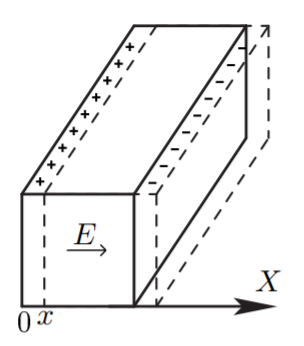
\includegraphics[scale=0.5]{2.png}
\end{wrapfigure}  
\begin{equation}
	N_D = n\dfrac{4}{3}\pi r_D^2.
\end{equation}
Теперь выделим параллелепипед с плотностью $n$ электронов, сместим их на $x$. Возникнут поверхностные заряды $\sigma = nex$, поле от которых будет придавать электронам ускорение:
$$
	\dfrac{d^2x}{dt^2}=-\dfrac{eE}{m}=-\dfrac{4\pi n e^2}{m}x.
$$ 
Отсюда получаем \textit{плазменную (ленгмюровскую) частоту} колебаний электронов:
\begin{equation}
	\omega_p = \sqrt{\dfrac{4\pi ne^2}{m}}.
\end{equation}
\subsection*{Одиночный зонд}
При внесении в плазму уединённого проводника -- \textit{зонда} -- с потенциалом, изначально равным потенциалу точки плазмы, в которую его помещают, на него поступают токи электроннов и ионов:
\begin{equation}
	\begin{array}{c}
	I_{e0} = \dfrac{n \langle v_e \rangle}{4}eS,\\
	I_{i0} = \dfrac{n \langle v_i \rangle}{4}eS,
	\end{array}
\end{equation}
где $\langle v_e \rangle$ и $\langle v_i \rangle$ -- средние скорости электронов и ионов, $S$ -- площадь зонда, $n$ -- плотность электронов и ионов. Скорости электронов много больше скорости ионов, поэтому $I_{i0} \ll I_{e0}$. Зонд будет заряжаться до некоторого равновестного напряжения $-U_f$ -- \textit{плавающего потенциала}.\\
\begin{wrapfigure}{r}{5.5cm}
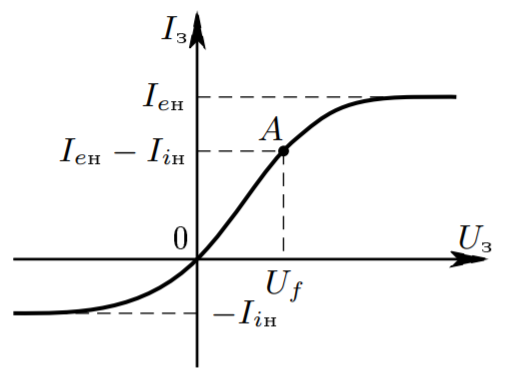
\includegraphics[scale=0.5]{3.png}
\end{wrapfigure}  
В равновесии ионный ток мало меняется, а электронный имеет вид
$$
	I_e = I_0 \exp\left( -\dfrac{eU_f}{kT_e} \right).
$$
Будем подавать потенциал $U_\text{з}$ на зонд и снимать значение зондового тока $I_\text{з}$. Максимальное значение тока $I_{e\text{н}}$ -- электронный ток насыщения, а минимальное $I_{i\text{н}}$ -- ионный ток насыщения. Значение из эмпирической формулы Бомона:
\begin{equation}
	I_{i\text{н}} = 0.4 neS \sqrt{\dfrac{2kT_e}{m_i}}.
\end{equation}
\subsection*{Двойной зонд}
Двойной зонд -- система из двух одинаковых зондов, расположенных на небольшом расстоянии друг от друга, между которыми создаётся разность потенциалов, меньшая $U_f$. Рассчитаем ток между ними вблизи $I=0$. При небольших разностях потенциалов ионные токи на оба зонда близки к току насыщения и компенсируют друг друга, а значит величина результирующего тока полностью связана с разностью электронных токов. Пусть потенциалы на зондах
$$
	U_1 = -U_f + \Delta U_1,
$$
$$
	U_2 = -U_f + \Delta U_2.
$$
Между зондами $U = U_2 - U_1 = \Delta U_2 - \Delta U_1$.
Через первый электрод
\begin{equation}
	I_1 = I_{i\text{н}} + I_{e1} = I_{i\text{н}} - \dfrac{1}{4}neS\langle v_e\rangle \exp\left(-\dfrac{eU_f}{kT_e}\right)\exp\left(\dfrac{e\Delta U_1}{kT_e}\right)=I_{i\text{н}}\left(1 - \exp\left( \dfrac{e\Delta U_1}{kT_e} \right)\right).
\end{equation}
Аналогично через второй получим
\begin{equation}
	I_2 = I_{i\text{н}}\left(1 - \exp\left( \dfrac{e\Delta U_2}{kT_e} \right)\right)
\end{equation}
  
Из $(7)$ и $(8)$ с учётом последовательного соединение зондов ($I_1 = -I_2 = I)$:
$$
	\Delta U_1= \dfrac{kT_e}{e}\text{ln}\left(1 - \dfrac{I}{I_{i\text{н}}}\right)
$$
$$
	\Delta U_2= \dfrac{kT_e}{e}\text{ln}\left(1 + \dfrac{I}{I_{i\text{н}}}\right)
$$

Тогда итоговые формулы для разности потенциалов и тока

\begin{equation}
	U = \dfrac{kT_e}{e}\text{ln}\dfrac{1 - I/I_{i\text{н}}}{1 + I/I_{i\text{н}}}, 
	I = I_{i\text{н}} \text{th}\dfrac{eU}{2kT_e}.
\end{equation}
Реальная зависимость выглядит несколько иначе и описывается формулой 
\begin{wrapfigure}{l}{7cm}
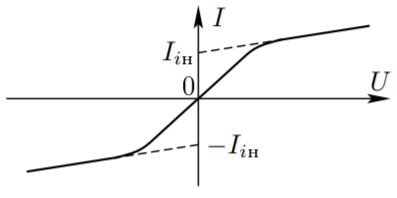
\includegraphics[scale=0.8]{4.png}
\vspace{+30pt}
\end{wrapfigure}
\begin{equation}
	I = I_{i\text{н}} \text{th}\dfrac{eU}{2kT_e} + AU.
\end{equation}
Из этой формулы можно найти формулу для $T_e$: для $U=0$ мы найдём $I_{i\text{н}}$, продифференцируем в точке $U=0$ и с учётом $\text{th}~\alpha \approx \alpha$ при малых $\alpha$ и $A\rightarrow 0$ получим:
\begin{equation}
	kT_e = \dfrac{1}{2}\dfrac{eI_{i\text{н}}}{\dfrac{dI}{dU}|_{U=0}}.
\end{equation}

\section{Экспериментальная установка}


\begin{center}
	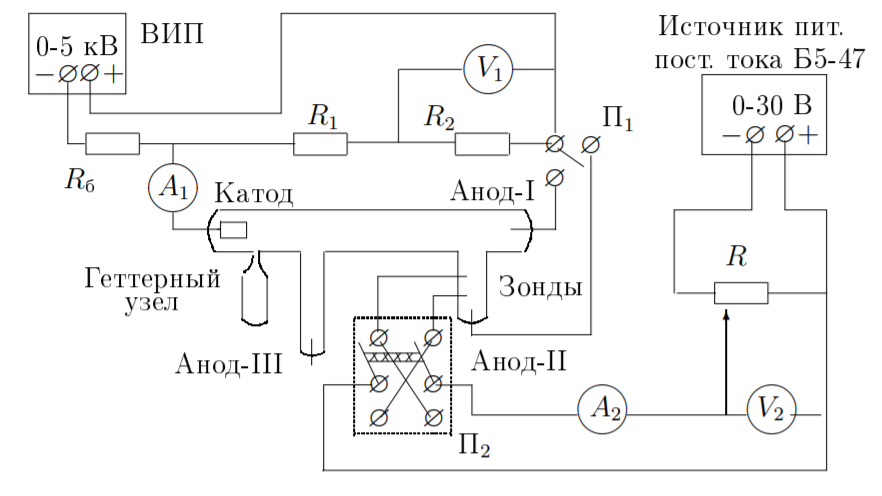
\includegraphics[scale=0.6]{1.png}
\end{center}

Стеклянная газоразрядная трубка имеет холодный (ненакаливаемый) полый катод, три анода и \textit{геттерный} узел -- стеклянный баллон, на внутреннюю повехность которого напылена газопоглощающая плёнка (\textit{геттер}). Трубка наполнена изотопом неона $^22$Ne при давлении 2 мм рт. ст. Катод и один из анодом (I и II) с помощью переключателя $\Pi_1$ подключается через балластный резистор $R_\text{б}$ ($\approx 450$ кОм) к регулируемому ВИП с выкодным напряжением до 5 кВ.

При подключении к ВИП анода-I между ним и катодом возникает газовый разряд. Ток разряда измеряется миллиамперметром $A_1$, а падение напряжения на разрядной трубке -- цифровым вольтметром $V_1$, подключённым к трубке черезе высокоомный (25 МОм) делитель напряжения с коэффициентом $(R_1+R_2)/R_2 = 10$.

При подключении к ВИП анода-II разряд возникает в пространстве между катодом и анодом-II, где находятся двойной зонд, используемый для диагностики плазмы положительного столба. Зонды изготовлены из молибденовой проволоки диаметром $d = 0.2$ мм и имеют длину $l = 5.2$ мм. Они подключены к источнику питания GPS через потенциометр $R$. Переключатель $\Pi_2$ позволяет изменять полярность напряжения на зондах. Величина напряжения на зондах изменяеься с помощью дискретного переключателя <<$V$>> выходного напряжения источника питания и потенциометра $R$, а измеряется цифровым вольтметром $V_2$. Для измерения зондового тока используется мультиметр $A_2$.


\section{{Ход работы}}

1) Подготовим приборы к работе. плавно увеличив выходное напряжение ВИП, определим напряжение зажигания($U_{\text{заж}} = 22,8$\ В)

2) С помощью вольтметра $V_1$ и амперметра $A_1$ снимем ВАХ $U_P(I_P)$. Данные представлены в таблице, приведенныой в конце.

3) Снимем ВАХ двойного зонда с помощью мультиметров $A_2$ и $V_2$ при $I_p = 5, 3, 1.5\ mA$.
Занесем в таблицу полученные данные (таблица привдена в конце). Построим графики

\begin{figure}[h]
    \centering
    \subfloat[ВАХ двойного зонда, $I = 5.0$ мА.]{{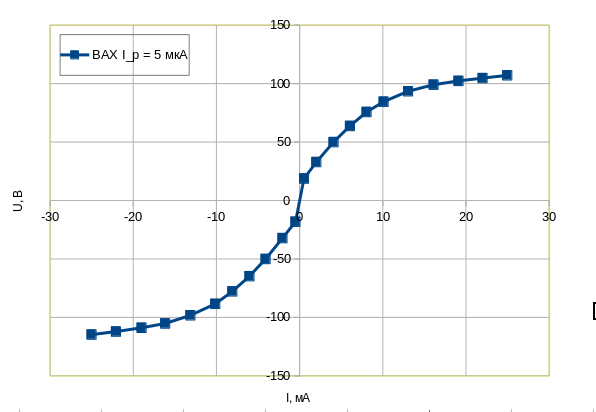
\includegraphics[width=0.5\textwidth]{6.png}}}
    \subfloat[ВАХ двойного зонда, $I = 3.0$ мА.]{{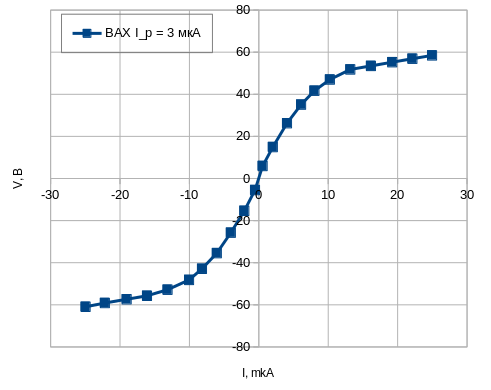
\includegraphics[width=0.5\textwidth]{7.png}}}\\
    \subfloat[ВАХ двойного зонда, $I = 1.5$ мА.]{{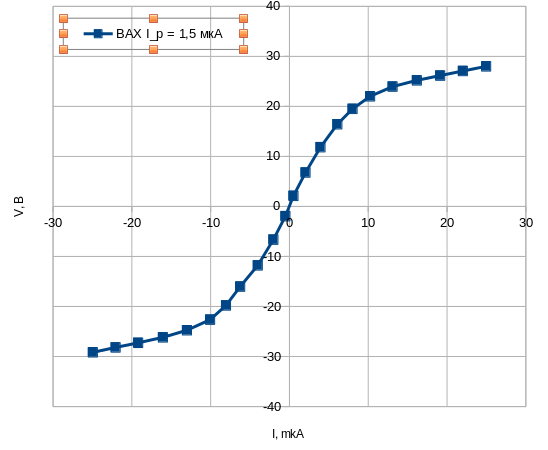
\includegraphics[width=0.5\textwidth]{8.png}}}
\end{figure}



\section{{Апроксимация полученных данных}}


\section{{Вывод}}


\section{{Список используемой литературы}}

$\bullet$ \href{https://vk.com/doc-139677307_612194888}{Никулин М.Г. Лабораторный практикум по общей физике. Электричество и магнетизм}\\

$\bullet$ \href{https://mipt.ru/education/chair/physics/S_III/lab_el.php}{Описание лабораторных работ на кафедре общей физики МФТИ}

$\bullet$ \href{https://vk.com/doc-139677307_612194961}{П.В. Попов, А.А. Нозик. Обработка результатов учебного эксперимента}

\begin{table}[h]
\centering
\begin{tabular}{|c|c|c|c|c|c|c|c|c|c|c|c|}
\hline
$U_p$, В & 48 & 61 & 71 & 81 & 90 & 100 & 110 & 120 & 130 & 140 & 150 \\ \hline
$I_p$, мА & 29.56 & 27.49 & 27.33 & 26.64 & 25.90 & 25.00 & 24.52 & 24.27 & 24.32 & 24.36 & 24.46  \\ \hline
\end{tabular}
\caption{Зависимость $U_P(I_P)$ в сторону увеличения\\.}
\end{table} 


\begin{table}[h]
\centering
\begin{tabular}{|c|c|c|c|c|c|}
\hline
$U_p$, В & 10 & 19 & 25 & 35 & 45 \\ \hline
$I_p$, мА & 35.12 & 24.48 & 33.90 & 32.98 & 30.72  \\ \hline
\end{tabular} 
\begin{tabular}{|c|c|c|c|c|c|c|c|c|c|c|}
\hline
$U_p$, В & 50 & 60 & 70 & 80 & 90 & 100 & 110 & 120 & 130 & 140 \\ \hline
$I_p$, мА & 28.96 & 27.63 & 27.26 & 26.66 & 26.40 & 25.12 & 24.68 & 24.38 & 24.34 & 24.34  \\ \hline
\end{tabular}
\caption{Зависимость $U_P(I_P)$ в сторону уменьшения\\.}
\end{table}

\begin{table}
\centering
\begin{tabular}{|c|c|c|c|c|c|c|c|}
\cline{1-2} \cline{4-5} \cline{7-8}

\multicolumn{2}{|c|}{$I_p = 5.0$ мА} &  & \multicolumn{2}{c|}{$I_p = 3.0$ мА} &  & \multicolumn{2}{c|}{$I_p = 1.5$ мА} \\ \cline{1-2} \cline{4-5} \cline{7-8} 

$U_2$, В & $I_2$, мкА &  & $U_2$, В & $I_2$, мкА &  & $U_2$, В & $I_2$, мкА \\ 
\cline{1-2} \cline{4-5} \cline{7-8}
 
 24.97 &  107.06 & &  24.96 &  58.46 & &  24.96 &  28.01 
 \\ \cline{1-2} \cline{4-5} \cline{7-8}
 22.00 &  104.70 & &  22.13 &  56.90 & &  22.01 &  27.08 
 \\ \cline{1-2} \cline{4-5} \cline{7-8}
 19.10 &  102.31 & &  19.22 &  55.24 & &  19.13 &  26.16 
 \\ \cline{1-2} \cline{4-5} \cline{7-8}
 16.11 &   99.04 & &  16.15 &  53.48 & &  16.17 &  25.21 
 \\ \cline{1-2} \cline{4-5} \cline{7-8}
 13.04 &   93.46 & &  13.18 &  51.18 & &  13.09 &  23.96 
 \\ \cline{1-2} \cline{4-5} \cline{7-8}
 10.10 &   84.50 & &  10.24 &  47.01 & &  10.24 &  22.02 
 \\ \cline{1-2} \cline{4-5} \cline{7-8}
  8.05 &   75.71 & &   8.01 &  41.69 & &   8.01 &  19.51 
 \\ \cline{1-2} \cline{4-5} \cline{7-8}
  6.05 &   63.77 & &   6.09 &  35.10 & &   6.08 &  16.44
 \\ \cline{1-2} \cline{4-5} \cline{7-8}
  4.08 &   49.95 & &   4.06 &  26.26 & &   3.94 &  11.85
 \\ \cline{1-2} \cline{4-5} \cline{7-8}
  2.01 &   32.88 & &   2.02 &  44.94 & &   2.04 &   6.78
 \\ \cline{1-2} \cline{4-5} \cline{7-8}
  0.53 &   18.74 & &   0.55 &   5.95 & &   0.51 &   2.12
 \\ \cline{1-2} \cline{4-5} \cline{7-8}
 -0.50 &  -18.19 & &  -0.55 &  -5.47 & &  -0.51 &  -1.94
 \\ \cline{1-2} \cline{4-5} \cline{7-8}
 -2.06 &  -32.18 & &  -2.09 & -15.34 & &  -2.04 &  -6.63 
 \\ \cline{1-2} \cline{4-5} \cline{7-8}
 -4.09 &  -50.01 & &  -4.03 & -25.73 & &  -4.02 & -11.78 
 \\ \cline{1-2} \cline{4-5} \cline{7-8}
 -6.03 &  -64.73 & &  -6.05 & -35.44 & &  -6.25 & -16.02 
 \\ \cline{1-2} \cline{4-5} \cline{7-8}
 -8.09 &  -77.76 & &  -8.19 & -42.88 & &  -8.05 & -19.79 
 \\ \cline{1-2} \cline{4-5} \cline{7-8}
-10.14 &  -88.44 & & -10.05 & -48.17 & & -10.07 & -22.63 
\\ \cline{1-2} \cline{4-5} \cline{7-8}
-13.13 &  -98.22 & & -13.15 & -52.81 & & -13.01 & -24.75 
\\ \cline{1-2} \cline{4-5} \cline{7-8}
-16.16 & -105.20 & & -16.11 & -55.71 & & -16.06 & -26.17 
\\ \cline{1-2} \cline{4-5} \cline{7-8}
-19.00 & -108.87 & & -19.04 & -57.36 & & -19.20 & -27.26 
\\ \cline{1-2} \cline{4-5} \cline{7-8}
-22.08 & -112.12 & & -22.18 & -59.12 & & -22.06 & -28.19 
\\ \cline{1-2} \cline{4-5} \cline{7-8}
-25.01 & -114.71 & & -24.96 & -60.94 & & -24.95 & -29.16 
\\ \cline{1-2} \cline{4-5} \cline{7-8}
\end{tabular}
\caption{Зависимость $U_3(I_3)$.}
\end{table} 
 

 













 




\end{document}